\documentclass[a4paper,12pt]{article}
\usepackage{graphicx}

\usepackage{epstopdf}
\usepackage{gensymb}
\usepackage{float}
\usepackage{mathtools}
\usepackage{setspace}
\usepackage{tabularx}
\title{Teknisk Dokumentation}
%% Definitioner för LIPS-dokument

\usepackage[swedish]{babel}
\usepackage[utf8]{inputenc}
\usepackage[T1]{fontenc}
\usepackage{times}
\usepackage{ifthen}
\usepackage[labelfont=it]{caption}

\usepackage[margin=25mm]{geometry}

\def\arraystretch{1.6}

\usepackage{fancyhdr}
\pagestyle{fancy}
\lhead{}
\chead{\LIPSprojekttitel}
\rhead{\LIPSdatum}
\lfoot{\LIPSkursnamn \\ \LIPSdokumentansvarig}
\rfoot{\LIPSprojektgrupp \\ \LIPSgruppepost}

\setlength{\parindent}{0pt}
\setlength{\parskip}{1ex plus 0.5ex minus 0.2ex}


\newcommand{\twodigit}[1]{\ifthenelse{#1<10}{0}{}{#1}}
\newcommand{\dagensdatum}{\number\year-\twodigit{\number\month}-\twodigit{\number\day}}

%% ------------------------------------------
% NYBILD
% Skapar centrerad bild med caption
%   
% #1: Filens url relativt '/bilder/'
% #2:  Caption
% #3: Label
% #4: Skalning i förhållande till textwidth
%% ------------------------------------------
\newcommand{\nyBild}[4] 
{\begin{figure}[H]
  \centering
 \emph{\includegraphics[angle=0,width=#4\textwidth]{bilder/#1}}
  \caption{\emph{#2}}
  \label{fig:#3}
\end{figure}}

%%  Redefinitions of commands containing @
\makeatletter
\makeatother

\newcommand{\LIPStitelsida}{%
{\ }\vspace{45mm}
\begin{center}
  \textbf{\Huge {\sffamily \LIPSdokumenttyp}}
\end{center}
\begin{center}
  {\Large \LIPSredaktor}
\end{center}
%\begin{center}
%  {\Large Version \LIPSversion}
%\end{center}
\vspace{60mm}
%\begin{center}
%  {\large Status}\\[1.5ex]
%  \begin{tabular}{|*{3}{p{40mm}|}}
%    \hline
%    Granskad & \LIPSgranskare & \LIPSgranskatdatum \\
%    \hline
%    Godkänd & \LIPSgodkannare & \LIPSgodkantdatum \\
%    \hline
%  \end{tabular}
%\end{center}
\newpage
}


\newenvironment{LIPSprojektidentitet}{%
{\ }\vspace{45mm}
\begin{center}
  {\Large PROJEKTIDENTITET}\\[0.5ex]
  {\small
  \LIPSprojektgrupp, \LIPSartaltermin, \LIPSprojekttitel\\
  Tekniska högskolan vid Linköpings universitet, ISY
  }
\end{center}
\begin{center}
  \begin{tabular}{|l|p{45mm}|p{25mm}|l|}
    \hline
    \textbf{Namn} & \textbf{Ansvar} & \textbf{Telefon} & \textbf{E-post} \\
    \hline
}
{
    \hline
  \end{tabular}
\end{center}
\begin{center}
  {\small
    \textbf{E-postlista för hela gruppen}: \LIPSgruppepost\\
    \textbf{Kontaktperson hos kund}: \LIPSkundkontakt\\
    \textbf{Kursansvarig}: \LIPSkursansvarig\\
    \textbf{Handledare}: \LIPShandledare\\
  }
\end{center}
\newpage
}
\newcommand{\LIPSgruppmedlem}[4]{\hline {#1} & {#2} & {#3} & {#4} \\}



\newenvironment{LIPSdokumenthistorik}{%
\begin{center}
  Dokumenthistorik\\[1ex]
  \begin{small}
    \begin{tabular}{|l|l|p{60mm}|l|l|}
      \hline
      \textbf{Version} & \textbf{Datum} & \textbf{Utförda förändringar} & \textbf{Utförda av} & \textbf{Granskad} \\
      }%
    {%
      \hline
    \end{tabular}
  \end{small}
\end{center}
}
\newcommand{\LIPSversionsinfo}[5]{\hline {#1} & {#2} & {#3} & {#4} & {#5} \\}



\newenvironment{packed_itemize}{
\begin{itemize}
	\setlength{\itemsep}{1pt}
    \setlength{\parskip}{0pt}
    \setlength{\parsep}{0pt}
}{\end{itemize}}

\newenvironment{packed_enumerate}{
\begin{enumerate}
	\setlength{\itemsep}{1pt}
    \setlength{\parskip}{0pt}
    \setlength{\parsep}{0pt}
}{\end{enumerate}}





%%% Local Variables: 
%%% mode: latex
%%% TeX-master: "kravspec_mall"
%%% End:

\usepackage{sectsty}
\allsectionsfont{\sffamily}

\frenchspacing

\renewcommand{\thepage}{\roman{page}}

\newcommand{\LIPSartaltermin}{VT14}
\newcommand{\LIPSkursnamn}{TSEA56 Elektronik kandidatprojekt}

\newcommand{\LIPSprojekttitel}{Lagerrobot}

\newcommand{\LIPSprojektgrupp}{Grupp 1}
\newcommand{\LIPSgruppepost}{tsea56-2014-grupp-1@googlegroups.com}
\newcommand{\LIPSdokumentansvarig}{LIPS Teknisk Dokumentation}

\newcommand{\LIPSkund}{ISY, Linköpings universitet, 581\,83 Linköping}
\newcommand{\LIPSkundkontakt}{Tomas Svensson, 013-28 13 68, tomass@isy.liu.se}
\newcommand{\LIPSkursansvarig}{Tomas Svensson, 013-28 13 68, 3B:528, tomass@isy.liu.se}
\newcommand{\LIPShandledare}{Anders Nilsson, 3B:512, 013-28 26 35, anders.p.nilsson@liu.se}


\newcommand{\LIPSdokumenttyp}{Teknisk Dokumentation}
\newcommand{\LIPSredaktor}{Karl Linderhed}
\newcommand{\LIPSversion}{1.0}
\newcommand{\LIPSdatum}{\dagensdatum}

\newcommand{\LIPSgranskare}{}
\newcommand{\LIPSgranskatdatum}{}
\newcommand{\LIPSgodkannare}{}
\newcommand{\LIPSgodkantdatum}{}

\begin{document}

\LIPStitelsida

%% Argument till \LIPSgruppmedlem: namn, roll i gruppen, telefonnummer, epost
\begin{LIPSprojektidentitet}
  \LIPSgruppmedlem{Karl Linderhed}{Projektledare (PL)}{073-679 59 59}{karli315@student.liu.se}
  \LIPSgruppmedlem{Patrik Nyberg}{Dokumentansvarig (DOK)}{073 -049 59 90}{patny205@student.liu.se}
  \LIPSgruppmedlem{Johan Lind}{}{070-897 58 24}{johli887@student.liu.se}
  \LIPSgruppmedlem{Erik Nybom}{}{070-022 47 85}{eriny778@student.liu.se}
  \LIPSgruppmedlem{Andreas Runfalk}{}{070-564 23 79}{andru411@student.liu.se}
  \LIPSgruppmedlem{Philip Nilsson}{}{073-528 48 86}{phini326@student.liu.se}
  \LIPSgruppmedlem{Lucas Nilsson}{}{073-059 42 94}{lucni395@student.liu.se}
\end{LIPSprojektidentitet}


\renewcommand*\contentsname{Innehåll}
\begin{spacing}{0.5}
\tableofcontents{}
\end{spacing}
\newpage

%% Argument till \LIPSversionsinfo: versionsnummer, datum, ändringar, utfört av, granskat av
%\addcontentsline{toc}{section}{Dokumenthistorik}
\begin{LIPSdokumenthistorik}
  \LIPSversionsinfo{1.0}{}{}{}{}
\end{LIPSdokumenthistorik}
\newpage

\renewcommand{\thepage}{\arabic{page}}
\setcounter{page}{1}

\section{Inledning}
\emph{Bakgrund och syfte}


\section{Produktbeskrivning}
\emph{En bild på produkten och en beskrivning av hur den fungerar.
Beskriv vad den används till.}

\section{Teori}
\emph{Beskrivning av regleralgoritmer m.m.}

\section{Systemöversikt}
\emph{Ett översiktligt blockschema och en beskrivning av hela systemet.}

\section{Gemensamma funktioner}
Detta avsnitt beskriver olika funktioner som inbegriper eller används av flera olika moduler.

\subsection{Protokoll för seriell kommunikation mellan robot och PC}
\label{sec:bt-protokoll}

\subsection{USART}
\label{sec:usart}
AVR-processorns inbyggda USART-funktionalitet används av flera delsystem. Därför finns ett gemensamt bibliotek med funktionalitet för att skicka och ta emot bytes över en seriell lina.

Biblioteket använder en byte-buffer för att lagra mottagen data. Till buffern hör två pekare, en läspekare och en skrivpekare, som pekar till olika element i buffern och flyttas upp när man läser eller skriver i buffern. Genom att pekarna endast kan anta värden mellan 0 och 255, samma antal värden som det finns element i buffern, fås funktionalitet som i en ringbuffer eftersom pekarnas värden svämmar över till 0 när de ökas från 255.

När avbrottet som indikerar att en byte har tagits emot kommer skrivs den byte som har tagits emot in i buffern på den position som skrivpekaren pekar på. Därefter ökas pekarens värde ett steg.

För att läsa en byte från buffern anropas funktionen \verb|usart_read_byte|. Den undersöker om det finns någon data tillgänglig som inte redan har lästs (med andra ord, om läs- och skrivpekaren skiljer sig från varandra). I sådana fall läser den in en byte från den position i buffern som läspekaren pekar på till en variabel, och stegar upp läspekaren med ett steg.

För att skicka data används funktionen \verb|usart_write_byte| som undersöker om den inbyggda USART-modulens statusflaggor tillåter att man skickar data, och i sådana fall ger en byte till USART-modulen som direkt matar ut den på den seriella linan.

\subsection{Intern buss}
\label{sec:bus}

\section{Sensorenhet}
\emph{Det här och de följande avsnitten innehåller mera detaljerade blockscheman och beskrivningar av varje modul.
Tänk på läsbarheten och växla mellan figurer och text.}
\section{Chassienhet}

\section{Armenhet}

\section{Kommunikationsenhet}
Kommunikationsenheten är robotens gränssnitt för interaktion med omvärlden och har två uppgifter. Den ska:
\begin{itemize}
\item agera som ett gränssnitt mot LCD-displayen och möjliggöra att alla delsystem kan skriva ut information på den.
\item hantera den seriella kommunikationen över Bluetooth och möjliggöra att roboten kan skicka och ta emot information till och från PC-gränssnittet.
\end{itemize}

\subsection{Seriell kommunikation över Bluetooth}
Anslutningen till datorn görs med bluetoothmodemet \emph{BlueSMiRF Gold} som är monterat på roboten. På PC-sidan skapas vid parkoppling med modemet en virtuell serieport, som emulerar en fysisk COM-port eller motsvarande. Kommunikationen sker sedan över denna port som om den vore en vanlig RS-232-port. 

På robotsidan används AVR-processorns inbyggda modul för UART, och det gemensamma biblioteket för USART som används av flera delsystem -- se avsnitt \ref{sec:usart}. Följande parametrar ställs in i det protokollet som roboten använder:
\begin{itemize}
\item Datahastigheten är 115 200 bps.
\item Data skickas som 8-bitars värden utan någon paritetsbit.
\item Ingen flödeshantering eller handskakning används.
\item Varje värde om 8 bitar avslutas med en stoppbit.
\end{itemize}

Hur olika typer av information överförs mellan robot och PC beskrivs närmare i avsnitt \ref{sec:bt-protokoll}.


\section{PC-gränssnitt}

\section{Slutsatser}
\emph{Vilka förbättringar skulle kunna göras?}

\newpage
\section*{Referenser}


\newpage
\appendix
\section{Kopplingsschema}
Robotens elektronik är uppdelad på två virkort. Därför presenteras här ett kopplingsschema för varje virkort.


\nyBild{kopplingsschema_sensor.pdf}{Kopplingsschema för virkortet som innehåller sensorenheten.}{senskoppling}{1}

\begin{figure}[H]
\centering
 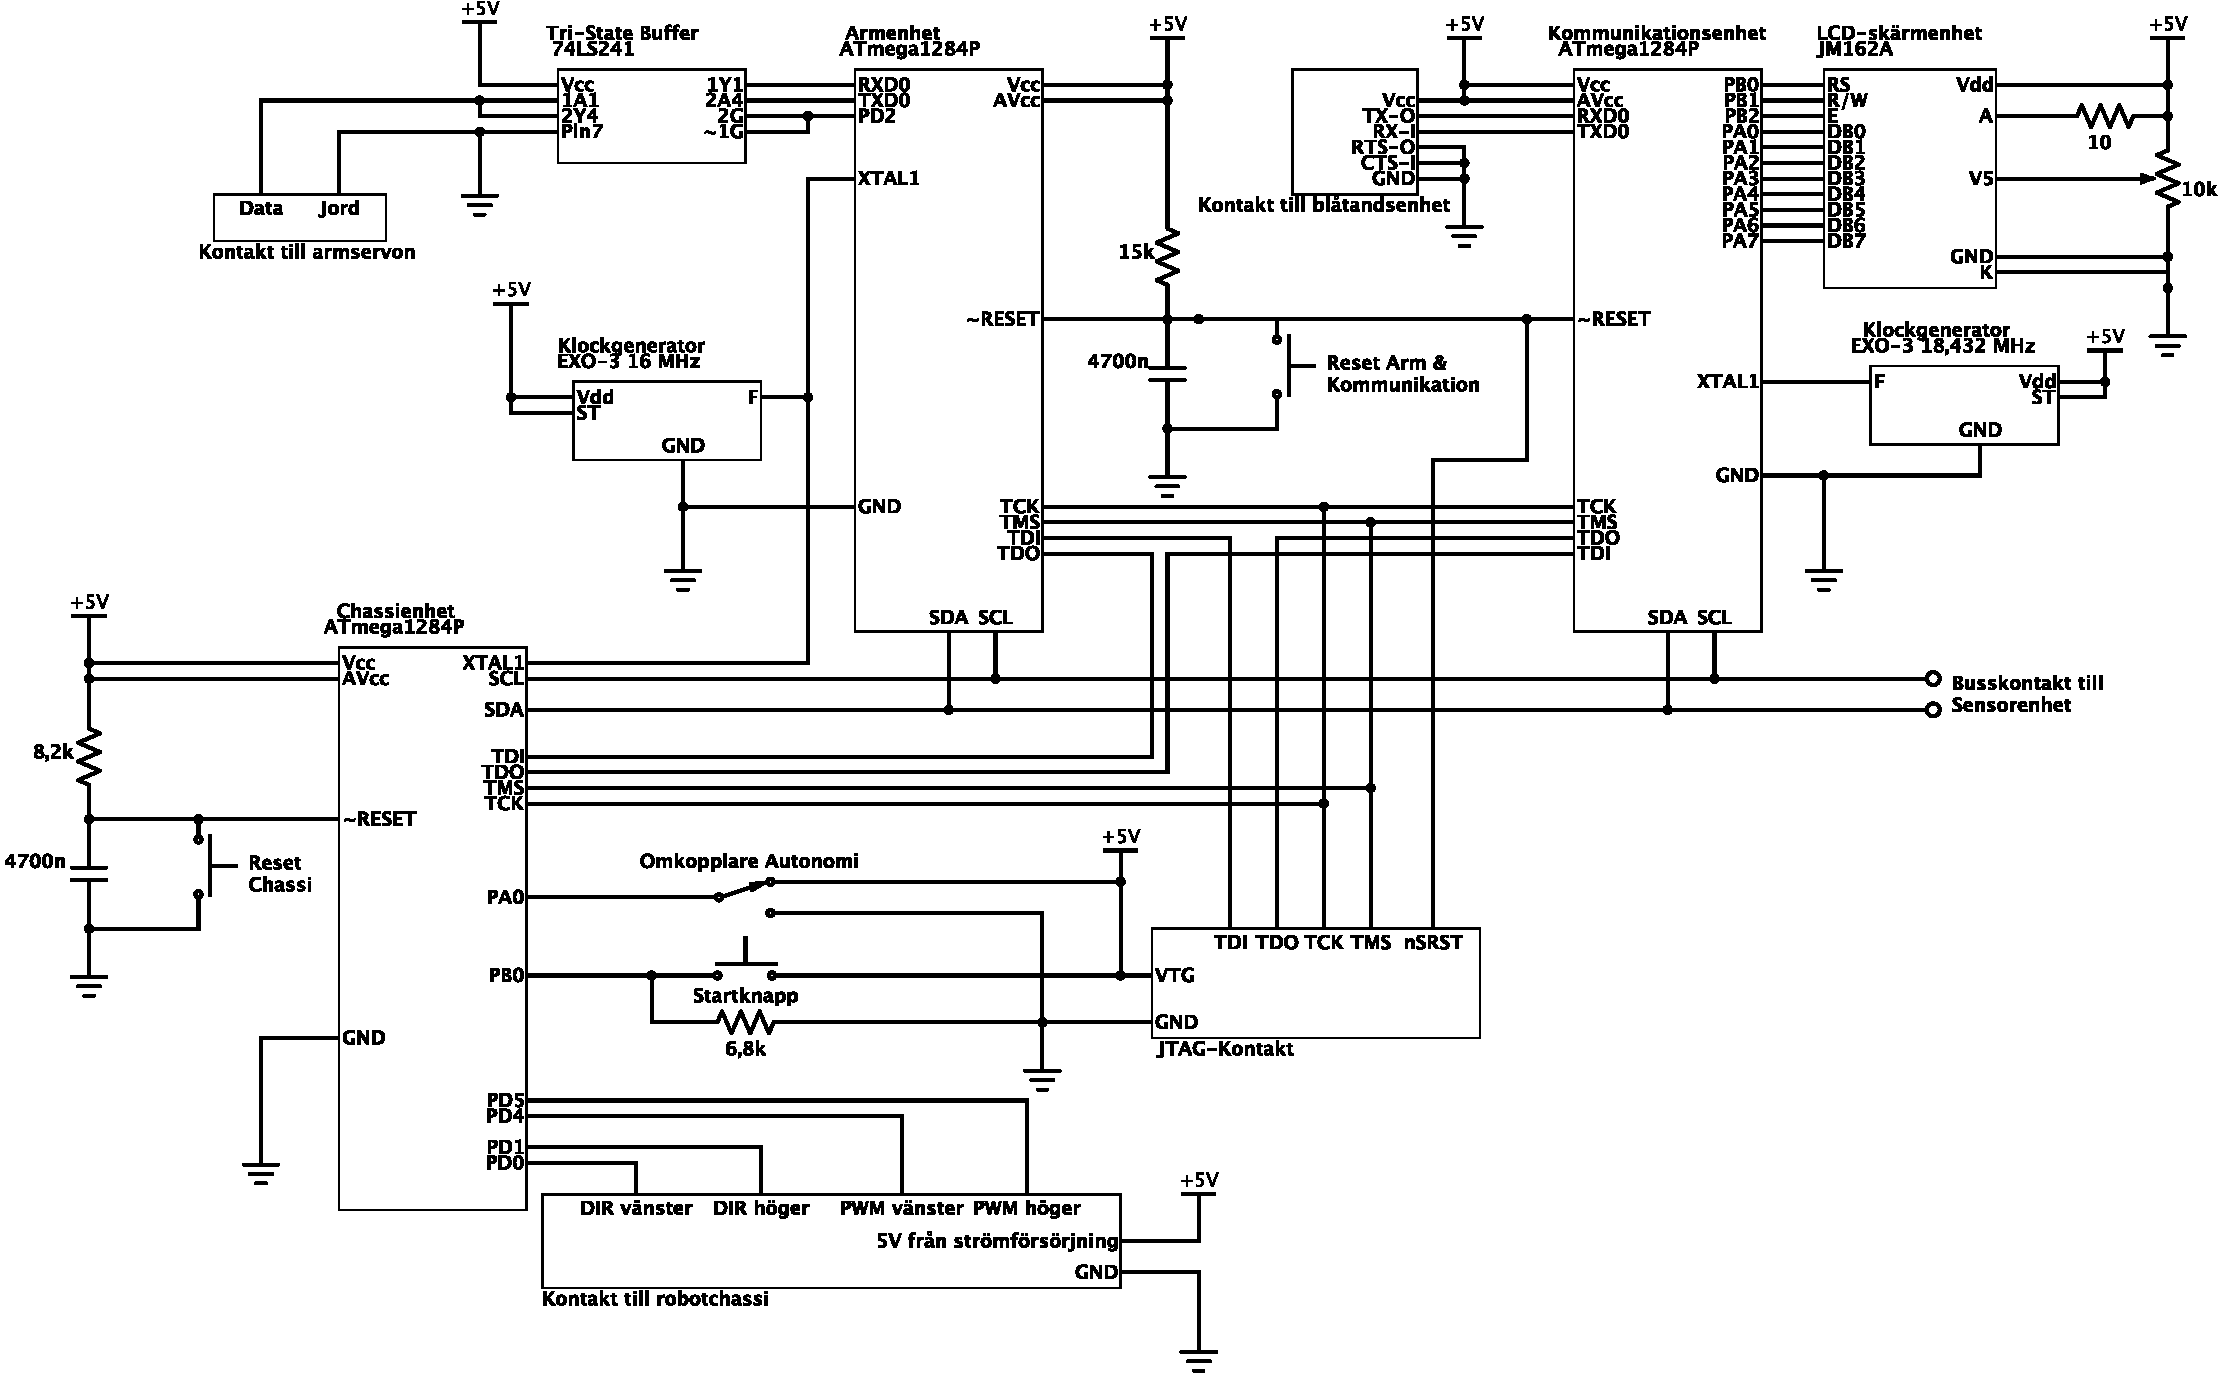
\includegraphics[angle=90,width=0.9\textwidth]{bilder/chassiarmkomm.pdf}
  \emph{\caption{Kopplingsschema över virkortet som innehåller kommunikationsenheten, chassienheten och armenheten.} \label{fig:chassiarmkomm}}
  
\end{figure}


\section{Utdrag från programlistning}
\emph{(ca 5-10 sidor så att vi kan bedöma kodens läsbarhet mm.) och eventuell VHDL-kod}
\section{Övriga bilagor?}


\end{document} 
